% Dit werk is gelicenseerd onder de licentie Creative Commons Naamsvermelding-GelijkDelen 4.0 Internationaal. Ga naar http://creativecommons.org/licenses/by-sa/4.0/ om een kopie van de licentie te kunnen lezen.
\documentclass[t]{beamer}

% vaak gebruikte packages, nederlands
\usepackage[margin=2.5cm]{geometry}     % Marges instellen
\usepackage[dutch]{babel}               % Voor nederlandstalige hyphenatie (woordsplitsing)
\usepackage{amsmath,amsthm}             % Uitgebreide wiskundige mogelijkheden
\usepackage{url}                        % Om url's te verwerken
\usepackage{graphicx,subfigure}         % Om figuren te kunnen verwerken
\usepackage{color}
\usepackage{framed}
\usepackage{multicol}
\usepackage[small,bf,hang]{caption}     % Om de captions wat te verbeteren
\usepackage[utf8]{inputenc}             % Om niet ascii karakters rechtstreeks te kunnen typen
\usepackage{float}                      % Om nieuwe float environments aan te maken. Ook optie H!
\usepackage{flafter}                    % Opdat floats niet zouden voorsteken
\usepackage[section]{placeins}			% Om ervoor te zorgen dat floats binnen dezelfde section blijven
\usepackage[nottoc]{tocbibind}			% Bibliografie en inhoudsopgave in ToC; zie tocbibind.dvi
\usepackage{fancyhdr}                   % Voor fancy headers en footers
\usepackage{thmtools}                   % theorem tools
\usepackage{parskip}                    % Om paragrafen met een verticale spatie ipv horizontaal te laten beginnen
\usepackage[plainpages=false]{hyperref} % Om hyperlinks te hebben in het pdfdocument.



%%%%%%%%%%%%%%%%%%%%%%%%%%%%%%
% Algemene instellingen van het document.
%%%%%%%%%%%%%%%%%%%%%%%%%%%%%%
\renewcommand{\baselinestretch}{1.2} 	% De interlinie afstand wat vergroten.
\setcounter{MaxMatrixCols}{50}          % Max 20 kolommen in een matrix


%%%%%%%%%%%%%%%%%%%%%%%%%%%%%%
% Headers en footers
%%%%%%%%%%%%%%%%%%%%%%%%%%%%%%
\pagestyle{fancy}
\fancyhf{}
\renewcommand{\headrulewidth}{0pt}
\fancyhead[RO] {\rightmark}
\fancyhead[LE] {\leftmark}
\fancyfoot[RO,LE] {\thepage}

% no dot after chapter number
\renewcommand{\chaptermark}[1]{
	\markboth{\MakeUppercase{ \chaptername\ \thechapter\quad #1}}{}
}
% no dot after section number
\renewcommand{\sectionmark}[1]{
	\markright{\MakeUppercase{ \thesection\quad #1}}{}
}

% page header and footer style in mainmatter aanpassen
\let\newmainmatter\mainmatter
\renewcommand{\mainmatter}{

	\pagestyle{fancy}
	\fancyhf{}
	\renewcommand{\headrulewidth}{0pt}
	\fancyhead[RO] {\rightmark}
	\fancyhead[LE] {\leftmark}
	\fancyfoot[RO,LE] {\thepage}
	\fancyfoot[C]{\tiny{Brecht Baeten}}

	\newmainmatter
}
\let\newappendix\appendix
\renewcommand{\appendix}{
	\fancyfoot{}
	\fancyfoot[RO,LE] {\thepage}
	\newappendix
}


%%%%%%%%%%%%%%%%%%%%%%%%%%%%%%
% Nieuwe omgevingen
%%%%%%%%%%%%%%%%%%%%%%%%%%%%%%
\definecolor{shadecolor}{gray}{0.95}
\newcounter{voorbeeldcounter}[chapter]
\renewcommand{\thevoorbeeldcounter}{\thechapter.\arabic{voorbeeldcounter}}
\makeatletter
\newenvironment{voorbeeld}
{
\vspace{3mm}
\addtolength{\leftskip}{5mm}
\begin{shaded*}
\vspace{-3mm}
\refstepcounter{voorbeeldcounter}
\noindent
\textbf{Voorbeeld \thevoorbeeldcounter:\\}
%\vspace{-8mm}
%\begin{multicols}{2}
}
{
%\end{multicols}
\end{shaded*}
\addtolength{\leftskip}{-5mm}
}
\makeatother  
    
%%%%%%%%%%%%%%%%%%%%%%%%%%%%%%
% .svg commando's
%%%%%%%%%%%%%%%%%%%%%%%%%%%%%%
% nieuw commando om svg files dynamisch te updaten
%\newcommand{\executeiffilenewer}[3]{%
%\ifnum\pdfstrcmp{\pdffilemoddate{#1}}%
%{\pdffilemoddate{#2}}>0%
%{\immediate\write18{#3}}\fi%
%}
%% nieuw commando om. svg figuren in te voegen
%% Gebruik: \includesvg{path/filename.svg}
%\newcommand{\includesvg}[2][0]{%
%\executeiffilenewer{#2.svg}{#2.pdf}%
%{inkscape -z -C --file=#2.svg %
%--export-pdf=#2.pdf --export-latex}%
%\ifx#10
%	\let\svgwidth\undefined
%\else
%	\def\svgwidth{#1}
%\fi%
%\input{#2.pdf_tex}%
%\ifx \svgwidth\undefined
%\else
%	\let\svgwidth\undefined
%\fi%
%}

% nieuw commando om .fig figuren in te voegen
\newcommand{\includefig}[2][0]{%
\ifx#10
	\let\figwidth\undefined
\else
	\def\figwidth{#1}
\fi%
\input{#2.pdf_tex}%
\ifx \figwidth\undefined
\else
	\let\figwidth\undefined
\fi%
}

%%%%%%%%%%%%%%%%%%%%%%%%%%%%%%
% Packages
%%%%%%%%%%%%%%%%%%%%%%%%%%%%%%

%\usepackage{geometry}              	% 
\usepackage[dutch]{babel}               % Voor nederlandstalige hyphenatie (woordsplitsing)
\uselanguage{dutch}
\languagepath{dutch}
\usepackage{amsmath,amsthm}             % Uitgebreide wiskundige mogelijkheden
\usepackage{url}                        % Om url's te verwerken
\usepackage{graphicx,subfigure}         % Om figuren te kunnen verwerken
\usepackage[utf8]{inputenc}             % Om niet ascii karakters rechtstreeks te kunnen typen
\usepackage[section]{placeins}			% Om ervoor te zorgen dat floats binnen dezelfde section blijven
\usepackage{multicol}
\usepackage[absolute,overlay]{textpos}

%%%%%%%%%%%%%%%%%%%%%%%%%%%%%%
% Layout
%%%%%%%%%%%%%%%%%%%%%%%%%%%%%%
\usetheme{Frankfurt}
\usefonttheme[onlymath]{serif}
\AtBeginSection[]
{
  \begin{frame}
    \frametitle{Inhoud}
    \tableofcontents[currentsection]
  \end{frame}
}

\setbeamertemplate{navigation symbols}{}
\setbeamertemplate{footline}[page number]

%%%%%%%%%%%%%%%%%%%%%%%%%%%%%%
% Title
%%%%%%%%%%%%%%%%%%%%%%%%%%%%%%
\title{Fluïdummechanica}
\author{Brecht Baeten\inst{1}}
\institute{
	\inst{1}%
  		KU Leuven, Technologie campus Diepenbeek,\\ e-mail: brecht.baeten@kuleuven.be
}
\date{\today}
%%%%%%%%%%%%%%%%%%%%%%%%%%%%%%
% Omgevingen
%%%%%%%%%%%%%%%%%%%%%%%%%%%%%%


\subtitle{Behoudsvergelijkingen langs stroomlijnen}

\begin{document}

	\frame{\titlepage}
	\section{Inleiding}
	\begin{frame}
		\frametitle{Voorbeeld}
		\center
    	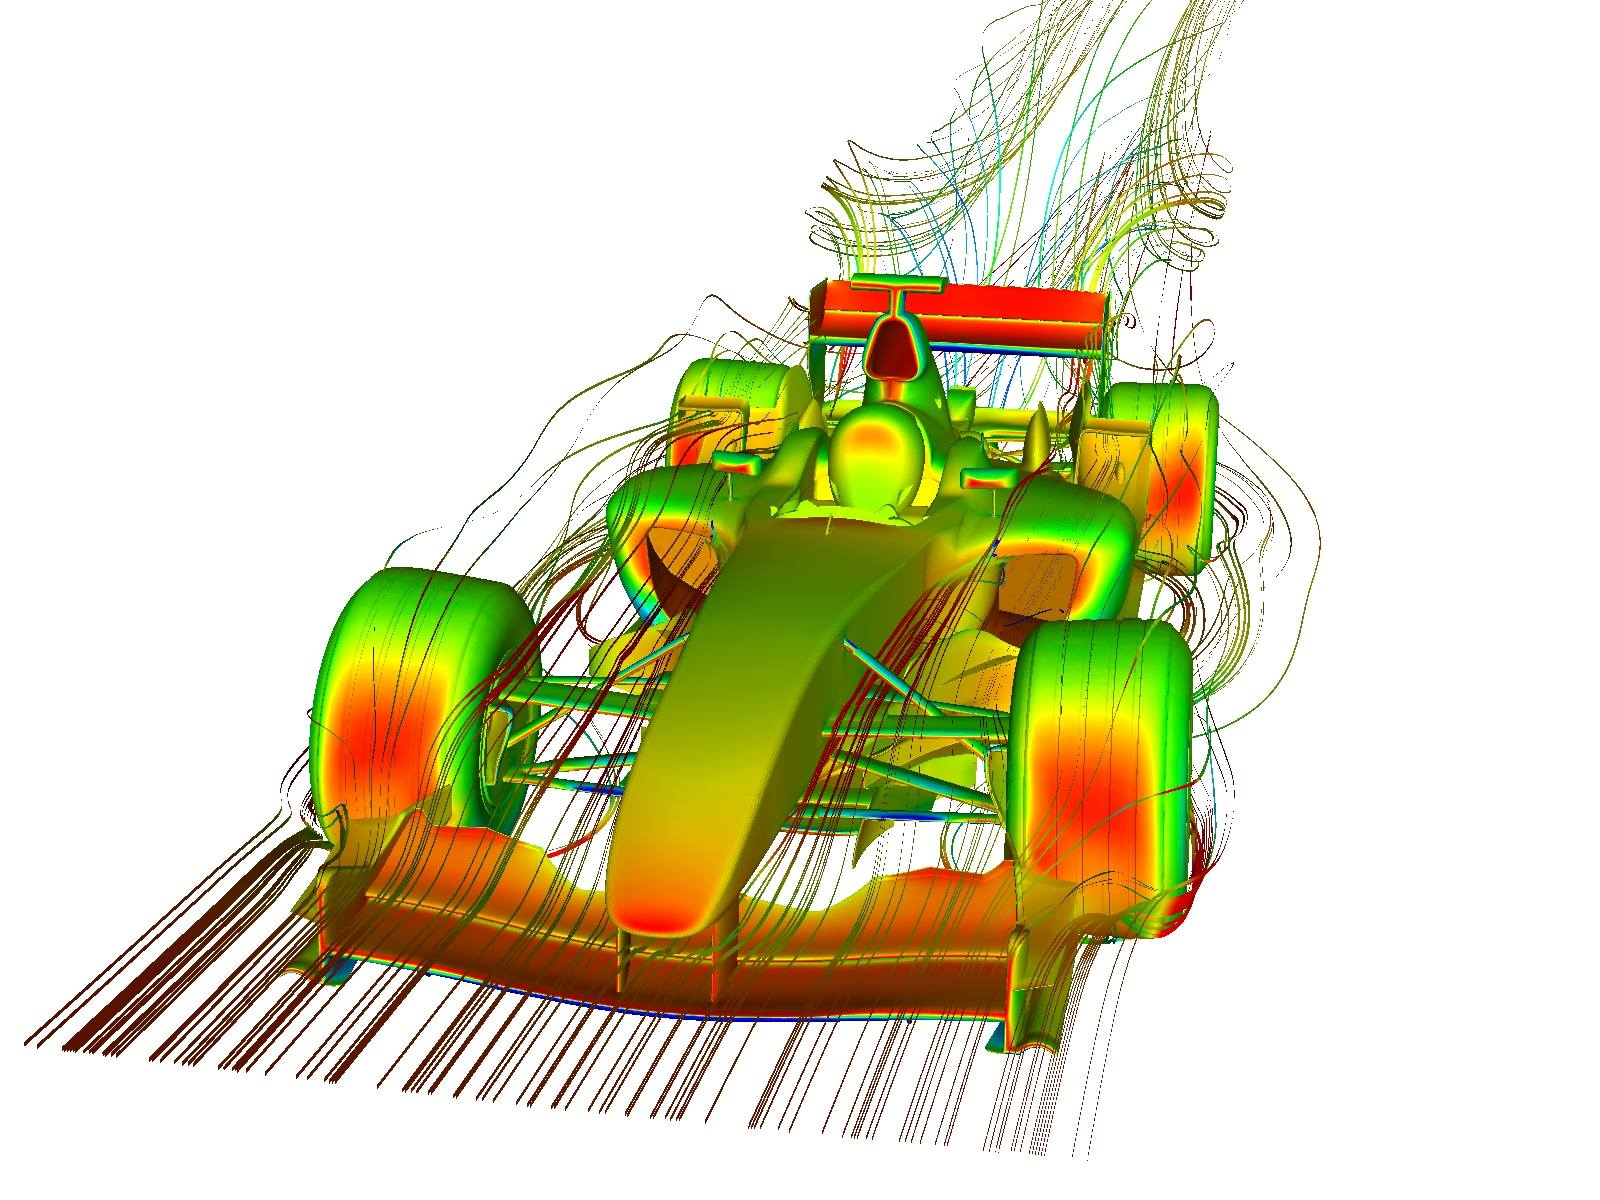
\includegraphics[height=0.8\textheight]{fig/deeltjesvergelijkingen/Dalco_Supercomputer_CFD_BMW_F1_PressurePath.jpg}\\
		\footnotesize{Bron: http://www.dalco.ch/}
  	\end{frame}
%%%%%%%%%%%%%%%%%%%%%%%%%%%%%%%%%%%%%%%%%%%%%%%%%%%%%%%%%%%%%%%%%%%%%%%%%%%
  	\section{Bewegingsvergelijking}	
  	\begin{frame}
		\frametitle{Stroomlijncoordinaten}
		\vspace{0.5cm}
		\centering
		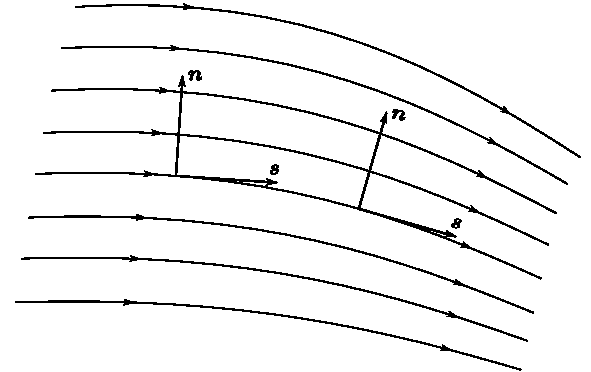
\includegraphics{fig/deeltjesvergelijkingen/Stoomlijncoordinaten}
  	\end{frame}
 %%%%%%%%%%%%%%%%%%%%%%%%%%%%%%%%%%%%%%%%%%%%%%%%%%%%%%%%%%%%%%%%%%%%%%%%%%%
  	\begin{frame}
		\frametitle{Bewegingsvergelijking}
		\vspace{0.5cm}
		\centering
		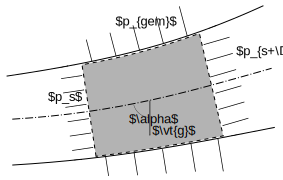
\includegraphics{fig/deeltjesvergelijkingen/Controlevolume_tussen_stroomlijnen}
  	\end{frame}
%%%%%%%%%%%%%%%%%%%%%%%%%%%%%%%%%%%%%%%%%%%%%%%%%%%%%%%%%%%%%%%%%%%%%%%%%%%
  	\begin{frame}
		\frametitle{Bewegingsvergelijking}
		\begin{textblock}{5}(0,3)
            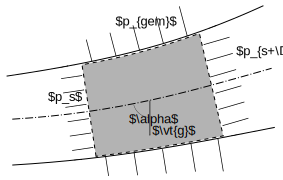
\includegraphics[width=5cm]{fig/deeltjesvergelijkingen/Controlevolume_tussen_stroomlijnen}
        \end{textblock}
        \only<1-3>{
        	\vspace{2.5cm}
        	\begin{equation*}
				\frac{\diff \vt{P}_{CV}}{\diff t} + \dot{\vt{P}}_{\partial CV} =  \vt{F}
        	\end{equation*}
        }
        \only<2-3>{
        	\begin{align*}
				\left. \rho v v_{\perp} A \right|_{s+\Delta s} - \left. \rho v v_{\perp} A \right|_{s} &= \left. p A \right|_{s} - \left. p A \right|_{s+\Delta s} \\
				&+ p_{gem} (\left. A \right|_{s+\Delta s}-\left. A \right|_{s}) -\rho g A_{gem} \Delta s \cos \alpha
        	\end{align*}
        }
        \only<3-3>{
        	\begin{align*}
				\frac{\left. \rho v v A \right|_{s+\Delta s} - \left. \rho v v A \right|_{s}}{\Delta s} &= -\frac{\left. p A \right|_{s+\Delta s} - \left. p A \right|_{s}}{\Delta s} \\
				& + p_{gem} \frac{\left. A \right|_{s+\Delta s}-\left. A \right|_{s}}{\Delta s} -\rho g A_{gem} \frac{\left. z\right|_{s+\Delta s} - \left. z\right|_{s}}{\Delta s}
			\end{align*}
		}
		\only<4-6>{
			\vspace{3.5cm}
			\begin{equation*}
				\frac{\diff \rho v v A}{\diff s} = -\frac{\diff p A}{\diff s} + p \frac{\diff A}{\diff s} -\rho g A \frac{\diff z}{\diff s}
			\end{equation*}
		}
		\only<5-6>{
			\begin{equation*}
				\rho v A \frac{\diff v}{\diff s} +  v \frac{\diff \rho v A}{\diff s} = -A \frac{\diff p}{\diff s} - p\frac{\diff A}{\diff s} + p \frac{\diff A}{\diff s} -\rho g A \frac{\diff z}{\diff s}
			\end{equation*}
		}
		\only<6-6>{
			\begin{equation}
				\rho v \frac{\diff v}{\diff s} + \frac{\diff p}{\diff s} + \rho g \frac{\diff z}{\diff s} = 0
				\label{eqn:vergelijking van Euler}
			\end{equation}
		}
  		\end{frame}
%%%%%%%%%%%%%%%%%%%%%%%%%%%%%%%%%%%%%%%%%%%%%%%%%%%%%%%%%%%%%%%%%%%%%%%%%%%
	\begin{frame}
		\frametitle{Deeltjesversnelling}
		\vspace{1cm}
		\begin{equation}
			\frac{\subsdiff}{\subsdiff t} = \frac{\partial}{\partial t} + v_x \frac{\partial}{\partial x} + v_y \frac{\partial}{\partial y} + v_z \frac{\partial}{\partial z}
		\end{equation}
		\pause
		\vspace{1cm}
		\begin{equation}
			\rho \frac{\subsdiff \vt{v}}{\subsdiff t} = -\nabla p + \rho \vt{g}
		\end{equation}
  	\end{frame}
%%%%%%%%%%%%%%%%%%%%%%%%%%%%%%%%%%%%%%%%%%%%%%%%%%%%%%%%%%%%%%%%%%%%%%%%%%%
	\section{Bernoulli}
	\begin{frame}
		\frametitle{Integratie van de bewegingsvergelijking}
		\vspace{1cm}
		\begin{equation*}
			\rho v \frac{\diff v}{\diff s} + \frac{\diff p}{\diff s} + \rho g \frac{\diff z}{\diff s} = 0
		\end{equation*}
		\pause
		\vspace{0.5cm}
		\begin{equation*}
			\int \rho v \frac{\diff v}{\diff s} \diff s + \int \frac{\diff p}{\diff s} \diff s + \int \rho g \frac{\diff z}{\diff s}  \diff s = \textrm{Cst}
		\end{equation*}
		\pause
        \hspace{5cm} $\Downarrow \quad \rho = \textrm{Cst}$ 
		\begin{equation}
			\frac{1}{2} \rho v^2 + p + \rho g z = \textrm{Cst}
			\label{eqn:vergelijking van Bernoulli}
		\end{equation}
  	\end{frame}
%%%%%%%%%%%%%%%%%%%%%%%%%%%%%%%%%%%%%%%%%%%%%%%%%%%%%%%%%%%%%%%%%%%%%%%%%%%
  	\begin{frame}
  		\frametitle{Bernoulli}
  		\begin{itemize}
  			\pause
  			\item Stationaire stroming
  			\pause
  			\item Langs een stroomlijn
  			\pause
  			\item Niet-viskeuze stroming
  			\pause
  			\item Niet-samendrukbare stroming
  		\end{itemize}
  		\pause
  		\vspace{1cm}
  		\begin{equation*}
			\frac{1}{2} \rho v^2 + p + \rho g z = \textrm{Cst}
		\end{equation*}
  	\end{frame}
%%%%%%%%%%%%%%%%%%%%%%%%%%%%%%%%%%%%%%%%%%%%%%%%%%%%%%%%%%%%%%%%%%%%%%%%%%%
	\begin{frame}
		\frametitle{Toepassing}
		Pitot-Statisch buis
		% demo
		\pause
		\vspace{0.5cm}
		\center
		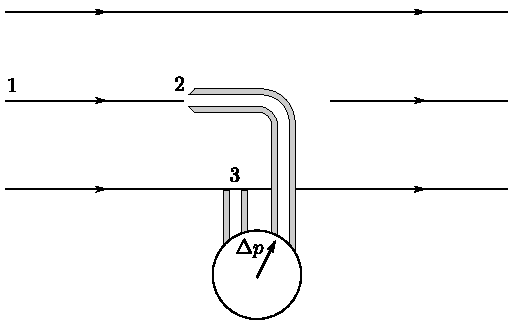
\includegraphics{fig/deeltjesvergelijkingen/Pitotstatischbuis}
	\end{frame}
%%%%%%%%%%%%%%%%%%%%%%%%%%%%%%%%%%%%%%%%%%%%%%%%%%%%%%%%%%%%%%%%%%%%%%%%%%%
	\begin{frame}
		\frametitle{Toepassing}
		\center
		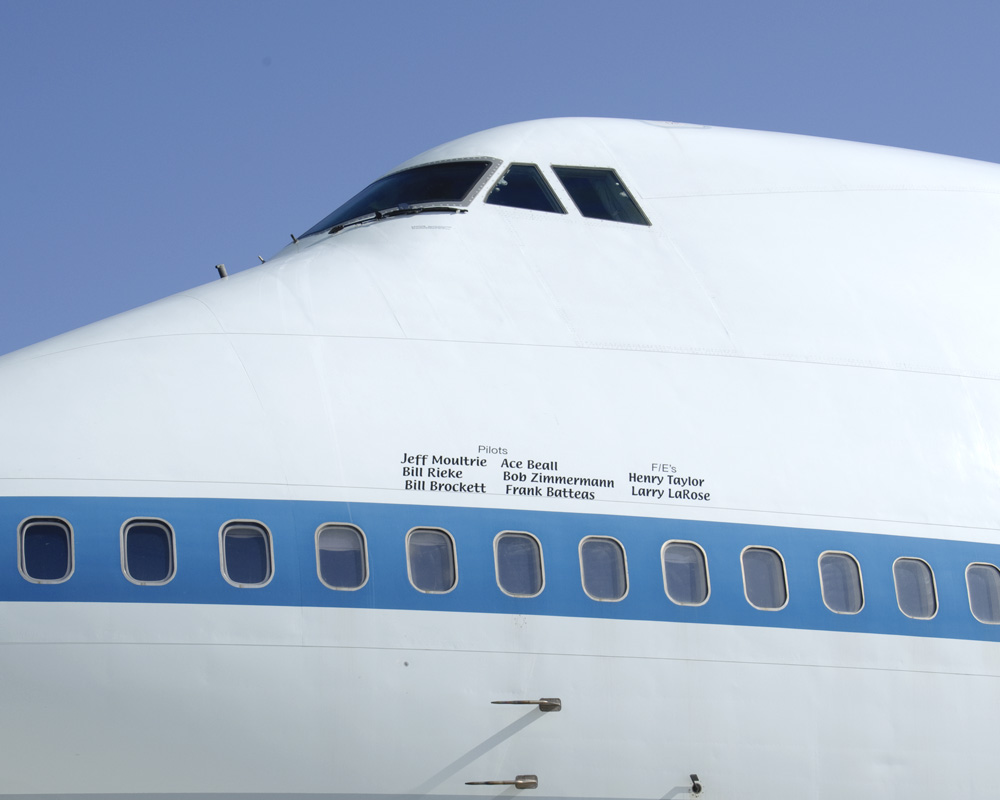
\includegraphics[height=0.8\textheight]{fig/deeltjesvergelijkingen/747pitottube}\\
		\footnotesize{Bron: http://www.edwardsflighttest.com/}
	\end{frame}
%%%%%%%%%%%%%%%%%%%%%%%%%%%%%%%%%%%%%%%%%%%%%%%%%%%%%%%%%%%%%%%%%%%%%%%%%%%
	\begin{frame}
		\frametitle{Mechanische arbeid van een deeltje}
		\begin{equation*}
			\rho v \frac{\diff v}{\diff s} = - \frac{\diff p}{\diff s} - \rho g \frac{\diff z}{\diff s}
		\end{equation*}
		\begin{equation*}
			W = \int_1^2 F \diff s
		\end{equation*}				
		\pause
		\begin{equation*}
			\int_1^2 \rho v \frac{\diff v}{\diff s} \diff s = - \int_1^2 \frac{\diff p}{\diff s} \diff s - \int_1^2 \rho g \frac{\diff y}{\diff s} \diff s
		\end{equation*}
		\pause
        \hspace{5cm} $\Downarrow \quad \rho = \textrm{Cst}$ 
        \begin{equation*}
			\rho \frac{1}{2} (v_2^2-v_1^2)  = - (p_2-p_1) - \rho g (z_2-z_1)
		\end{equation*}
		\pause
		\begin{equation}
			\rho \frac{1}{2} (v_2^2-v_1^2) + (p_2-p_1) + \rho g (z_2-z_1) = 0
			\label{eqn:kinetische energie en arbeid}
		\end{equation}
  		\end{frame}
%%%%%%%%%%%%%%%%%%%%%%%%%%%%%%%%%%%%%%%%%%%%%%%%%%%%%%%%%%%%%%%%%%%%%%%%%%%
	\begin{frame}
		\frametitle{Grafische voorstelling}
		\vspace{1cm}
		\center
		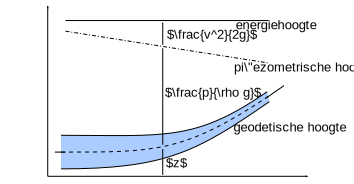
\includegraphics{fig/deeltjesvergelijkingen/Energiehoogte}
	\end{frame}
%%%%%%%%%%%%%%%%%%%%%%%%%%%%%%%%%%%%%%%%%%%%%%%%%%%%%%%%%%%%%%%%%%%%%%%%%%%
	\begin{frame}
		\frametitle{Energiebeschouwingen en irreversibiliteit}
		\begin{equation*}
			\dot{m} (u_u + \frac{p_u}{\rho_u} + \frac{1}{2}v^2_u + g z_u) - \dot{m} (u_i + \frac{p_i}{\rho_i}+ \frac{1}{2}v^2_i + g z_i) = \dot{Q}-\dot{W}_a
		\end{equation*}
		\pause
			\hspace{5cm} $\Downarrow \quad \rho = \textrm{Cst}, \dot{Q} = 0, \dot{W}_a = 0$ 
		\begin{equation*}
			u_u + \frac{p_u}{\rho} + \frac{1}{2}v^2_u + g z_u = u_i + \frac{p_i}{\rho}+ \frac{1}{2}v^2_i + g z_i
		\end{equation*}
		\pause
		\begin{equation*}
			\rho (u_u-u_i) + (p_u-p_i) + \frac{1}{2} \rho (v_u^2-v_i^2) + \rho g (z_u-z_i) = 0
		\end{equation*}
		\pause
		\begin{center}
			vs
		\end{center}
		\begin{equation*}
			(p_2-p_1) + \frac{1}{2} \rho (v_2^2-v_1^2) + \rho g (z_2-z_1) = 0
		\end{equation*}
	\end{frame}
%%%%%%%%%%%%%%%%%%%%%%%%%%%%%%%%%%%%%%%%%%%%%%%%%%%%%%%%%%%%%%%%%%%%%%%%%%%
	\section{Navier-Stokes}
	\begin{frame}
		\frametitle{Navier-Stokes vergelijking}
		\begin{itemize}
  			\item Newtoniaanse vloeistof
  			\item Niet-samendrukbare stroming
  		\end{itemize}
  		\pause
  		\vspace{1cm}
  		\begin{equation}
			\rho \frac{\subsdiff \vt{v}}{\subsdiff t} = -\nabla p + \rho \vt{g} + \mu \nabla^2 \vt{v}
		\end{equation}
		\pause
		\vspace{0.2cm}
		\begin{align}
			&\rho \left(\frac{\partial v_x}{\partial t} + v_x \frac{\partial v_x}{\partial x} + v_y \frac{\partial v_x}{\partial y} + v_z \frac{\partial v_x}{\partial z} \right) = \nonumber\\
			&\hspace{2cm} -\frac{\partial p}{\partial x} +\rho g_x + \mu \left( \frac{\partial^2 v_x}{\partial x^2} + \frac{\partial^2 v_x}{\partial y^2} + \frac{\partial^2 v_x}{\partial z^2} \right)
		\end{align}
	\end{frame}
	\begin{frame}
		\frametitle{Continuiteitsvergelijking}
		\begin{textblock}{5}(0,3)
            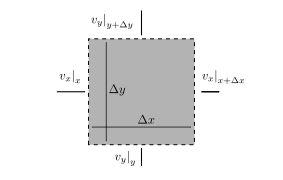
\includegraphics[width=5cm]{fig/deeltjesvergelijkingen/Continuiteitsvergelijking}
        \end{textblock}
  		\pause
  		\vspace{1.5cm}
  		\begin{align*}
			0 &= (\rho v_x|_{x} - \rho v_x|_{x+\Delta x})\Delta y \Delta z \\
			  &+ (\rho v_y|_{y} - \rho v_y|_{y+\Delta y})\Delta x \Delta z \\
			  &+ (\rho v_z|_{z} - \rho v_z|_{z+\Delta z})\Delta x \Delta y
		\end{align*}
		\pause
		\begin{equation*}
			0 = \frac{\rho v_x|_{x} - \rho v_x|_{x+\Delta x}}{\Delta x} + \frac{\rho v_y|_{y} - \rho v_y|_{y+\Delta y}}{\Delta y} + \frac{\rho v_z|_{z} - \rho v_z|_{z+\Delta z}}{\Delta z}
		\end{equation*}
		\pause
		\begin{equation*}
			\frac{\partial \rho v_x}{\partial x} + \frac{\partial \rho v_y}{\partial y} + \frac{\partial \rho v_z}{\partial z} = 0
		\end{equation*}
		\pause
		\begin{equation}
			\vt{\nabla} \vt{v} = 0
		\end{equation}
	\end{frame}	
%%%%%%%%%%%%%%%%%%%%%%%%%%%%%%%%%%%%%%%%%%%%%%%%%%%%%%%%%%%%%%%%%%%%%%%%%%%
\end{document}			